%図や表現の確認
\chapter{用語の説明}

本章では音楽用語の定義及びその説明を行う。

\section{音}

音とは、弾性体~(空気)~中を伝播する弾性波により起こされる音波が聴覚により感じられるもののことである。また、音波に周期性があり明確な音程を持つ音として聞こえる場合は楽音と呼ばれる。

\section{楽音の三要素}

楽音は高さ,大きさ,音色の三つの要素~(音の三要素)~から成り立っているとされる。

\begin{description}

\item[音の高さ]\mbox{}

\begin{figure}[t]
\begin{center}
\begin{minipage}{0.48\hsize}
\begin{center}
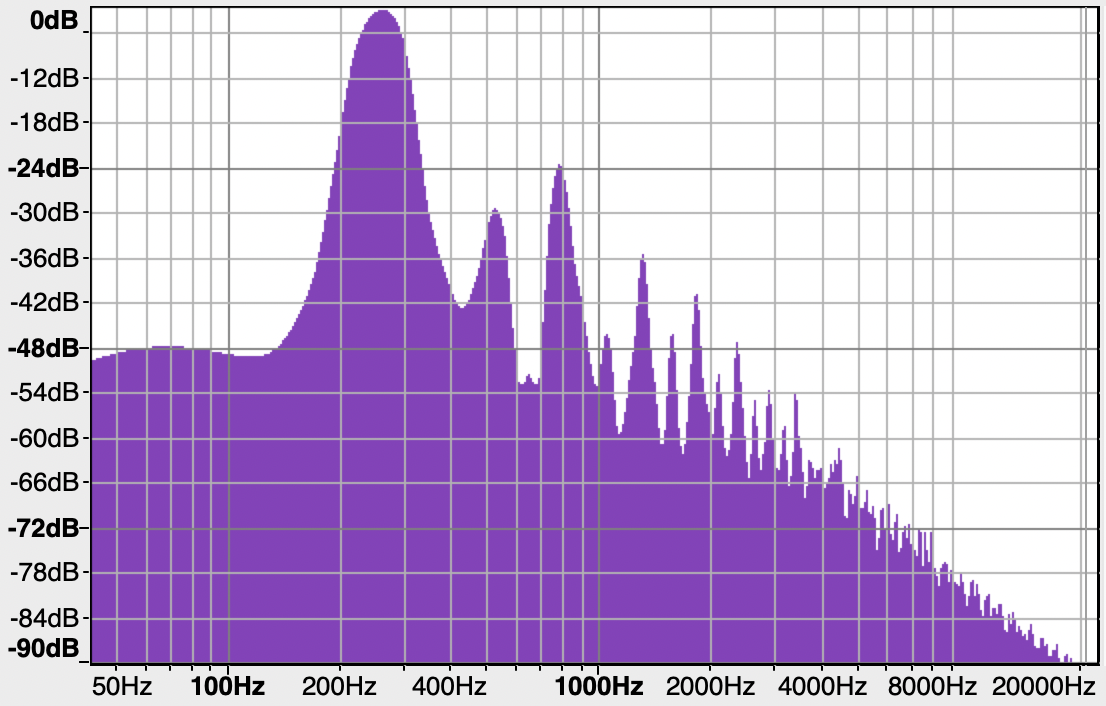
\includegraphics[width=0.95\hsize]{figure/c4_harp_spectrum.png}
\caption{ハープの音波のスペクトル}
\label{fig:spectrum}
\end{center}
\end{minipage}
\begin{minipage}{0.48\hsize}
\begin{center}
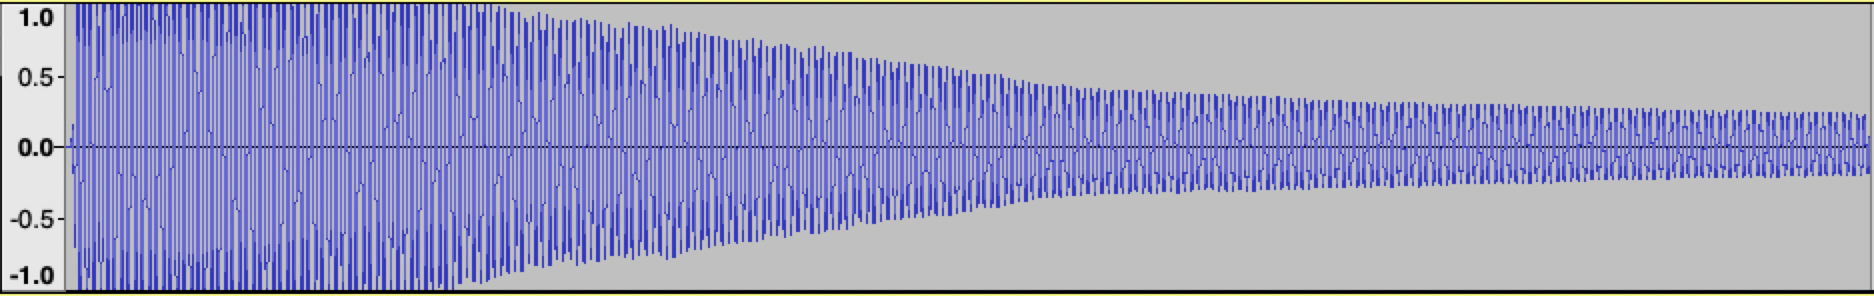
\includegraphics[width=0.95\hsize]{figure/c4_harp_wav.png}
\caption{ハープの音波の波形}
\label{fig:wav}
\end{center}
\end{minipage}
\end{center}
\end{figure}

音の高さは音波の周波数により決まる。一般には、フーリエ変換によりスペクトル分析を行った際の最も低い周波数成分の音波の周波数~(基音)~を音の高さと呼ぶ。また、図\ref{fig:spectrum}は図\ref{fig:wav}で示される音波のスペクトルであり、基音が264Hzとなる。

\item[音の大きさ]\mbox{}

\begin{figure}[t]
\begin{center}
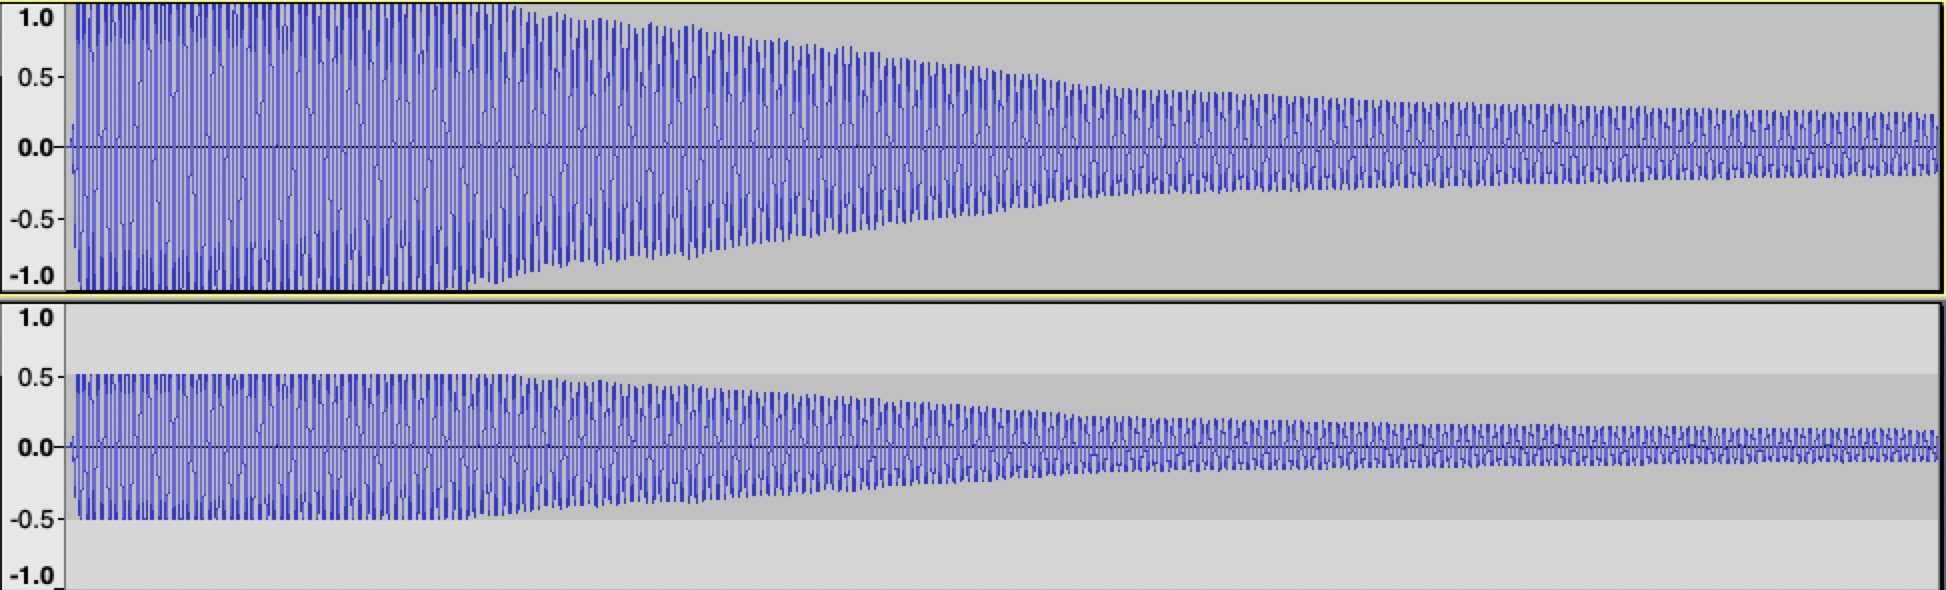
\includegraphics[width=0.7\hsize]{figure/c4_harp_loudness.png}
\caption{音の大きさの異なるハープの音波}
\label{fig:loudness}
\end{center}
\end{figure}

音の大きさは音波の振幅により決まる。図\ref{fig:loudness}では同じ楽器から出る同じ高さの音の音波を示しているが、振幅の大きい後者の方が音の大きさは大きい。

\item[音の音色]\mbox{}

\begin{figure}[t]
\begin{center}
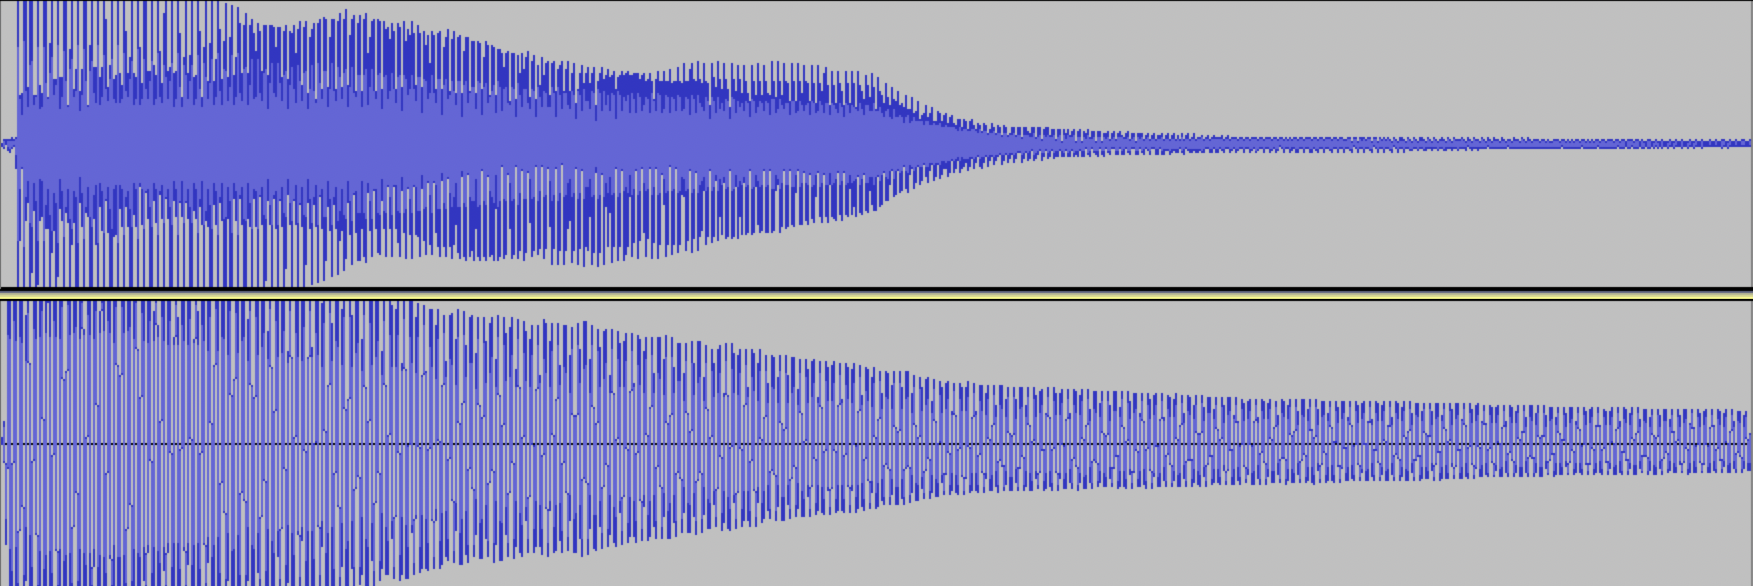
\includegraphics[width=0.7\hsize]{figure/c4_guitar_harp.png}
\caption{ギターとハープの音色の比較}
\label{fig:guitar_harp_comp}
\end{center}
\end{figure}

音の高さと大きさが同じであっても異なった音として知覚される時の違いを音色と呼ぶ。図\ref{fig:guitar_harp_comp}は上側はギターの音波,下側はハープの音波で同じ高さかつ同じ大きさであるが、このような音波の波形の違いが音色の違いを作り出す。

\end{description}